\begin{exercice*}
    Construire quatre triangles égaux à $PIC$ ayant pour côté $[OU]$. 

    Utiliser quatre couleurs distinctes pour les côtés des triangles différents de $[OU]$.

    \hspace*{-1cm}
    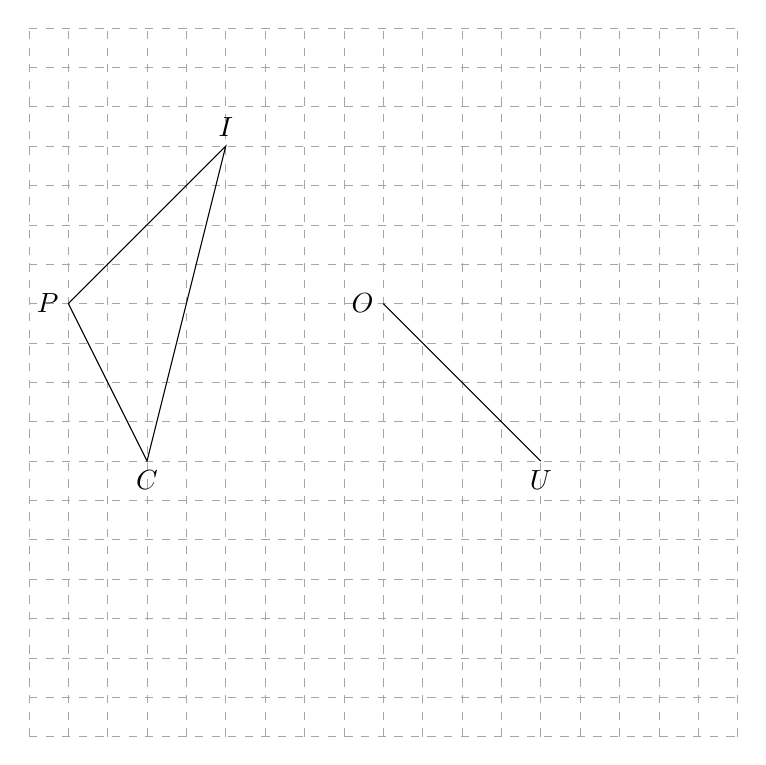
\begin{tikzpicture}[scale = 0.5]
        \draw[help lines, color=gray!70, dashed] (0,0) grid (18,18);
        \coordinate[label=left:$P$] (P) at (1,11);
        \coordinate[label=above:$I$] (I) at (5,15);
        \coordinate[label=below:$C$] (C) at (3,7);        
        \coordinate[label=left:$O$] (O) at (9,11);
        \coordinate[label=below:$U$] (U) at (13,7);
        \draw (P) -- (I) -- (C) -- (P);   
        \draw (O) -- (U);
        % \coordinate[label={[red]left:$S_1$}] (S1) at (5,9);
        % \draw[color=red] (O) -- (S1) -- (U);
        % \coordinate[label={[blue]below:$S_2$}] (S2) at (11,3);
        % \draw[color=blue] (O) -- (S2) -- (U);
        % \coordinate[label={[myGreen]right:$S_3$}] (S3) at (17,9);
        % \draw[color=myGreen] (O) -- (S3) -- (U);
        % \coordinate[label={above:$S_4$}] (S4) at (11,15);
        % \draw (O) -- (S4) -- (U);
    \end{tikzpicture}

\end{exercice*}
\begin{corrige}
    %\setcounter{partie}{0} % Pour s'assurer que le compteur de \partie est à zéro dans les corrigés
    \phantom{rrr}    

    \begin{tikzpicture}[scale = 0.5]
        \draw[help lines, color=gray!70, dashed] (0,0) grid (18,18);
        \coordinate[label=left:$P$] (P) at (1,11);
        \coordinate[label=above:$I$] (I) at (5,15);
        \coordinate[label=below:$C$] (C) at (3,7);        
        \coordinate[label=left:$O$] (O) at (9,11);
        \coordinate[label=below:$U$] (U) at (13,7);
        \draw (P) -- (I) -- (C) -- (P);   
        \draw (O) -- (U);
        \coordinate[label={[red]left:$S_1$}] (S1) at (5,9);
        \draw[color=red] (O) -- (S1) -- (U);
        \coordinate[label={[blue]below:$S_2$}] (S2) at (11,3);
        \draw[color=blue] (O) -- (S2) -- (U);
        \coordinate[label={[myGreen]right:$S_3$}] (S3) at (17,9);
        \draw[color=myGreen] (O) -- (S3) -- (U);
        \coordinate[label={above:$S_4$}] (S4) at (11,15);
        \draw (O) -- (S4) -- (U);
    \end{tikzpicture}
\end{corrige}

